\begin{frame}
  \frametitle{Analysis}
	\begin{itemize}
		\item Analyzes incoming samples, low-pass filtering them.
		\item Output in form of a natural number, which determines the height of the bars.
		\item Updates in synd with vsync.
		\item Both left & right channel separately.
	\end{itemize}
\end{frame}

\begin{frame}
  \frametitle{Analysis}
	\begin{figure}[h]
		\centering
			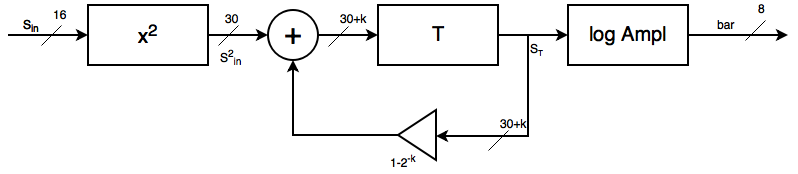
\includegraphics[width=16cm]{lowpass}
			\caption{The low-pass filter. $k$ is chosen by the approximation $\frac{1}{10}\mathrm{\ s} = 2^k\cdot\frac{1}{48800}\Rightarrow 2^k=4880\approx 2^{12}\Rightarrow k = 12 $}
			\label{fig:lowpass}
\end{figure}
\end{frame}
